\documentclass[10pt]{article}
\usepackage[polish]{babel}
\usepackage[utf8]{inputenc}
\usepackage[T1]{fontenc}
\usepackage{amsmath}
\usepackage{amsfonts}
\usepackage{amssymb}
\usepackage[version=4]{mhchem}
\usepackage{stmaryrd}
\usepackage{graphicx}
\usepackage[export]{adjustbox}
\graphicspath{ {./images/} }

\begin{document}
\begin{enumerate}
  \item Znajdź wszystkie czwórki liczb naturalnych \(a, b, c, d\) spełniające równanie
\end{enumerate}

\[
a b+b c+a c=a b c d
\]

\begin{enumerate}
  \setcounter{enumi}{1}
  \item Wykaż, że trójka \((0,0,0)\) jest jedynym rozwiązaniem w liczbach całkowitych równania
\end{enumerate}

\[
x^{3}=2 y^{3}+4 z^{3}
\]

\begin{enumerate}
  \setcounter{enumi}{2}
  \item W półkole o promieniu 5 wpisano trzy przystające prostokąty, jak na rysunku poniżej. Jakie pole ma jeden taki prostokąt?\\
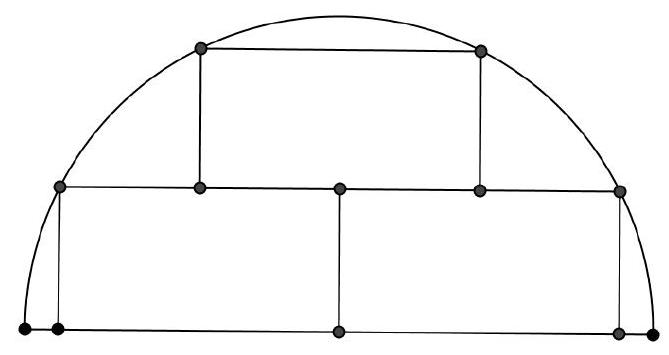
\includegraphics[max width=\textwidth, center]{2024_11_21_9a8810d60a17513d82e4g-1}
\end{enumerate}

\end{document}